Una unidad de memoria es un conjunto de celdas de almacenamiento junto con los circuitos asociados que se requieren para transferir información al y del dispositivo. El tiempo que toma transferir información a o de cualquier posición al azar deseada siempre es el mismo, de ahí el nombre memoria de acceso aleatorio o RAM

Una unidad de memoria almacena información binaria en grupos de bits llamados \textbf{palabras}. Una palabra de memoria es una \textit{entidad de bits que siempre se guardan o sacan juntos}, como una unidad. Una palabra de memoria es un \textit{grupo de unos y ceros y podría representar un número, una instrucción, uno o más caracteres alfanuméricos o cualquier otra información codificada en binario}. Un grupo de ocho bits es un byte. Casi todas las memorias de computadora manejan palabras \textbf{cuya longitud es un múltiplo de ocho bits}. Así, una palabra de 16 bits contiene dos bytes, y una de 32 bits consta de cuatro bytes. La capacidad de una unidad de memoria por lo regular se da como el número total de bytes que es capaz de guardar.

\subsection{Comunicación con la Memoria}
La comunicación entre la memoria y su entorno se efectúa a través de líneas de entrada y salida de datos, líneas de selección de direcciones y líneas de control que especifican la dirección de la transferencia.

Las $n$ líneas de entrada de datos alimentan la información que se guardará en la memoria, y las $n$ líneas de salida de datos proporcionan la información que viene de la memoria. Las $k$ líneas de dirección especifican la palabra específica escogida, de entre muchas disponibles. Las dos entradas de control especifican la dirección de la transferencia deseada: la entrada de escritura hace que se transfieran datos binarios a la memoria; la de lectura hace que se saquen datos binarios de la memoria.

\begin{figure}[h]
\centering
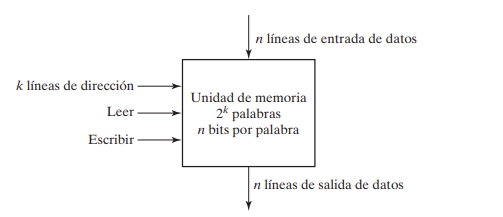
\includegraphics[scale=0.95]{img/mem.png}
\caption{Diagrama de bloques - Unidad de Memoria}
\end{figure}

La unidad de memoria se especifica con el número de palabras que contiene y el número de bits que hay en cada palabra. Las líneas de dirección seleccionan una palabra específica. A cada palabra de la memoria se asigna un número de identificación, llamado dirección, entre $0$ y $2^k -1$, donde $k$ es el número de líneas de dirección. La selección de una palabra específica de la memoria se efectúa aplicando los $k$ bits de dirección a las líneas de dirección. Un decodificador acepta esta dirección y abre las trayectorias necesarias para seleccionar la palabra especificada.

Para nombrar a las memorias, se suele decir que es de una capacidad y de tantos bits. La capacidad de palabras (o bytes) de la memoria se da con letras tales como: $K$ (kilo), $M$ (mega), $G$ (giga), $T$ (tera). $K$ es igual a $2^{10}$, $M$ es igual a $2^{20}$, $G$ es igual a $2^{30}$ y $T$ es igual a $2^{40}$.

\begin{mdframed}[backgroundcolor=gray!10,linewidth=0]
    Por ejemplo, la unidad de memoria con capacidad de 1K palabras de 16 bits cada una. Puesto que 1K=1024=210 y 16 bits constituyen dos bytes, se afirma que la memoria puede dar cabida a 2048=2K bytes.
\end{mdframed}

\newpage
El diagrama correspondiente a una memoria de $1K$ palabras de $16$ bits cada una se muestra en la figura \ref{fig:memfoto}.
\begin{figure}[h]
\centering
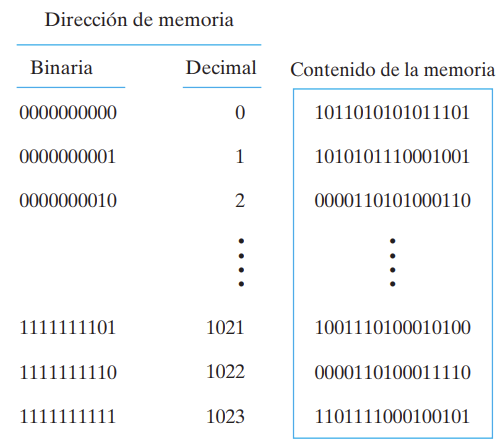
\includegraphics[scale=0.7]{img/ejem.png}
\caption{Contenido de una memoria de 1024 x 16}
\label{fig:memfoto}
\end{figure}

Cada palabra contiene 16 bits que se
dividen en dos bytes. Las palabras se reconocen por su dirección decimal, de 0 a 1023. La dirección binaria equivalente consta de 10 bits. La primera dirección se especifica con 10 ceros, y la última, con 10 unos. Ello se debe a que 1023 en binario es 1111111111. Seleccionamos una palabra de memoria por su dirección binaria. Cuando se lee o escribe una palabra, la memoria opera sobre los 16 bits como una sola unidad.

\begin{mdframed}[backgroundcolor=gray!10,linewidth=0]
    La memoria de $1K \times 16$ de la figura \ref{fig:memfoto} tiene $10$ bits en la dirección y $16$ bits en cada palabra.
\end{mdframed}